\TChapter{Análisis y diseño}{delta}
\ \\\\
En este capítulo se describe el análisis y el diseño del trabajo propuesto para
la recolección y clasificación de noticias.

%------------------------Requisitos Funcionales ------------------%
\section[Requisitos f.]{Requisitos funcionales}

%----------------------------RF1------------------------------%
   \Dline{RF1}{Recolectar noticias}
    \begin{itemize}
      \item \textbf{Descripción:} El sistema debe recolectar noticias de forma automática en Internet.\\
    \end{itemize}
%----------------------------RF2------------------------------%
   \Dline{RF2}{Clasificar noticias}
    \begin{itemize}
      \item \textbf{Descripción:} El sistema debe clasificar las noticias recolectadas de acuerdo a su contenido.\\
    \end{itemize}
%----------------------------RF3------------------------------%
   \Dline{RF3}{Mostrar resultados}
    \begin{itemize}
      \item \textbf{Descripción:} El sistema mostrará las URLs de las noticias que cumplan con los criterios de búsqueda establecidos.\\
    \end{itemize}


%------------------------Requisitos No Funcionales ---------------%
\section[Requisitos no f.]{Requisitos no funcionales}



%----------------------------RNF1------------------------------%
   \DVline{RNF1}{Tiempo de clasificación}
    \begin{itemize}
      \item \textbf{Descripción:} La clasificación de una noticia no debe tardar mas de cinco segundo.\\
    \end{itemize}

%----------------------------RNF2------------------------------%
   \DVline{RNF2}{Número de palabras}
    \begin{itemize}
     \item \textbf{Descripción:} Las noticias recolectads deberán tener un mínimo de 180 palabras en ellas.\\
    \end{itemize}

%----------------------------RNF3------------------------------%  
   \DVline{RNF3}{Número de noticias mostradas}
    \begin{itemize}
      \item \textbf{Descripción:} En el sitio web, se den visualizar almenos 15 noticias.\\
    \end{itemize}

%----------------------------RNF4------------------------------%  
   \DVline{RNF4}{Tiempo de actualización}
    \begin{itemize}
      \item \textbf{Descripción:} El tiempo para mostrar las 15 noticias clasificadas no debe exceder los 3 segundos.\\
    \end{itemize}


%----------------------------Reglas de negocio---------------------%  
\section{Reglas de negocio}


En esta sección se describen las reglas de negocio implementadas en el trabajo propuesto.\\\\
%------------------RN1-----------------------%
\DGline{RN1}{Número de palabras}
\begin{itemize}
  \item \textbf{Tipo:}  
  \item \textbf{Descripción:}  La notica debe tener almenos 180 palabras
  \item \textbf{Ejemplo:}
  \item \textbf{Refer:}
\end{itemize}
%------------------RN2-----------------------%
\DGline{RN2}{Lenguaje de direcciones web}

\begin{itemize}
  \item \textbf{Tipo:}  
  \item \textbf{Descripción:} Las direcciones de los sitios a consultar deben estar redactadas en lenguaje español.
  \item \textbf{Referenciado por:} \Tref{CU1}{CU1 Seleccionar sección} \\
\end{itemize}
%------------------RN3-----------------------%
\DGline{RN3}{Lenguaje de noticias}

\begin{itemize}
  \item \textbf{Tipo:}  
  \item \textbf{Descripción:} Las noticias deben estar redactadas en lenguaje español mexicano.
  \item \textbf{Ejemplo:}
  \item \textbf{Referenciado por:}  \\
\end{itemize}
%------------------RN4-----------------------%
\DGline{RN4}{Restricción en la recoleción}

\begin{itemize}
  \item \textbf{Tipo:}  
  \item \textbf{Descripción:} Solo se puede recoletar información de los sitios que lo permitan.
  \item \textbf{Ejemplo:}
  \item \textbf{Referenciado por:}  \\
\end{itemize}
%------------------RN5-----------------------%
\DGline{RN5}{Porcentaje de aceptación}

\begin{itemize}
  \item \textbf{Tipo:}  
  \item \textbf{Descripción:} Solo se puede mostrar una noticia si cumple con un porcentaje de aceptación mayor a 60\%.
  \item \textbf{Ejemplo:}
  \item \textbf{Referenciado por:}  \\
\end{itemize}
%------------------RN6-----------------------%
\DGline{RN6}{Formato de fecha}

\begin{itemize}
  \item \textbf{Tipo:} Derivación.
  \item \textbf{Descripción:} El formato de fecha se define como:\\

  $F=D/M/A$

  $donde$\\ 

  $D=\{x/x\ E\ N,1\leq\ x\ \leq31\}$\\
  $M=\{y/y\ E\ N,1\leq\ y\ \leq12\}$\\
  $A=\{z/z\ E\ N,1990\leq\ z\ \leq\Lambda_i\}$\\

  $F:Fecha$\\
  $\Lambda_i:Anio\_actual$\\

  \item \textbf{Ejemplo:} 
  \item \textbf{Referenciado por:} \Tref{CU2}{CU2 Buscar noticias} \\
\end{itemize}

%------------------RN7-----------------------%
\DGline{RN7}{Perido preestablecido}

\begin{itemize}
  \item \textbf{Tipo:} Cálculo
  \item \textbf{Descripción:} El formato de fecha es el descrito en la \RNref{RN6}{Formato de fecha}; El periodo preestablecido se define de la siguiente forma.\\\\
  \textbf{Fecha fin}:Toma el valor de la fecha actual.\\
  \textbf{Fecha inicio}: Es colocada 5 día antes de la fecha actual; Se muestra la forma completa para el cálculo del día, mes y año:\\
  $Sea$\\
  $D_a:Dia\_actual$\\
  $M_a:Mes\_actual$\\
  $A_a:Anio\_actual$\\
  $F_i:Fecha\_inicio$\\
  $mod:Operacion\ modulo$\\
  $\Psi(M_a):Funcion\ dias\ de \ mes$\\

  $\xi=\frac{D_a-5}{\mid D_a-5 \mid}$\\

  $\delta=\frac{\xi(\mid\xi-1\mid)}{2}$\\

  La fecha toma el sigueinte valor:\\
  $F_i=D_c/M_c/A_c$\\ 
  Existen 4 casos para calcular el día, mes y años; Dependen del mes y el día actual: \\

  \begin{tabular}{|l|c|c|}
  	\hline
	\multicolumn{1}{| >{\columncolor{black}}l|}{ \textcolor{myWhite}{\textbf{Caso:}} }&
	\multicolumn{1}{| >{\columncolor{black}}c|}{ \textcolor{myWhite}{1} }&\multicolumn{1}{| >{\columncolor{black}}c|}{ \textcolor{myWhite}{2} }\\
	\hline
	\textbf{Restricción:}&$2\leq\ M_a\leq\ 12;D_a\neq5$  &$2\leq\ M_a\leq\ 12;D_a=5$\\
	\hline 
	\textbf{$D_c:$}&$(D_a-5)\pmod{\Psi(M_a-1)+1}$   &$\Psi(M_a-1)$\\
	\hline
	\textbf{$M_c:$}&$M_a+\delta$        			 &$M_a-1$\\
	\hline
	\textbf{$A_c:$}&$A_a$        				     &$A_a$\\
	\hline
  \end{tabular}


  \begin{tabular}{|l|c|c|}
  	\hline
	\multicolumn{1}{| >{\columncolor{black}}l|}{ \textcolor{myWhite}{\textbf{Caso:}} }&
	\multicolumn{1}{| >{\columncolor{black}}c|}{ \textcolor{myWhite}{3} }&\multicolumn{1}{| >{\columncolor{black}}c|}{ \textcolor{myWhite}{4} }\\
	\hline
	\textbf{Restricción:}&$M_a=1;D_a \neq 5$&\ \ \ \ \ \ $M_a=1;D_a=5$\ \ \ \ \ \\
	\hline 
	\textbf{$D_c:$}&\ \ \ \ \ \ \ \ \ $(D_a-5)\pmod{32}$\ \ \ \ \ \ \ \ & $31$\\
	\hline
	\textbf{$M_c:$}&$\xi\pmod{13}$&$12$\\
	\hline
	\textbf{$A_c:$}&$A_a+\delta$&$A_a-1$\\
	\hline
  \end{tabular}


  \item \textbf{Ejemplo:} 
  \item \textbf{Referenciado por:} \Tref{CU1}{CU1 Seleccionar sección}, \Tref{CU2}{CU2 Buscar noticias} \\
\end{itemize}%------------------RN8-----------------------%
\DGline{RN8}{Periodo válido}

\begin{itemize}
  \item \textbf{Tipo:} Derivación.
  \item \textbf{Descripción:}\\
  $Sea$\\

  $F_i:Fecha\_inicio$\\
  $F_f:Fecha\_fin$\\

  $T=\{Valido,Invalido\}$\\
  $\psi\ \epsilon\ T$\\

  Un periodo de fecha se defino como:\\

  $(\psi=Valido)\leftrightarrow(F_i\ \leq\ F_f)$\\
  $(\psi=Invalido)\leftrightarrow(F_i\ >\ F_f)$\\
  \item \textbf{Ejemplo:}
  \item \textbf{Referenciado por:} \Tref{CU2}{CU2 Buscar noticias} \\
\end{itemize}
%------------------RN9-----------------------%
\DGline{RN9}{Límite de periodo}

\begin{itemize}
  \item \textbf{Tipo:} Derivación. 
  \item \textbf{Descripción:} 

  $Sea$\\

  $F_i:Fecha\_inicio$\\
  $F_f:Fecha\_fin$\\
  $F_a:Fecha\_actual$\\
  $F_c:01/01/1990$\\

  $T=\{Valido,Invalido\}$\\
  $\psi\ \epsilon\ T$\\

  $\Phi=[F_c,F_a]$\\
  $I=[F_i,F_f]$\\
  

  Un intervalo de tiempo dentro de los limites del sistema se define como:\\

  $(\psi=Valido)\leftrightarrow(I\ \subseteq\ \Phi)$\\
  $(\psi=Invalido)\leftrightarrow(I\ \nsubseteq \Phi)$\\

  \item \textbf{Referenciado por:} \Tref{CU2}{CU2 Buscar noticias} \\
\end{itemize}

%------------------RN10-----------------------%
\DGline{RN10}{Campos obligatorios}

\begin{itemize}
  \item \textbf{Tipo:} Restricción.  
  \item \textbf{Descripción:} Los campos marcados con \* no se deben omitir.
  \item \textbf{Ejemplo:} 
  \item \textbf{Referenciado por:}  \\
\end{itemize}
%------------------RN11-----------------------%
\DGline{RN11}{Sitios restringidos}

\begin{itemize}
  \item \textbf{Tipo:}m
  \item \textbf{Descripción:} No se debe acceder a las siguientes páginas:
    \begin{itemize}
        \item Facebook
        \item Youtube
        \item Twitter
        \item Instagram 
    \end{itemize} 
  \item \textbf{Ejemplo:}
  \item \textbf{Referenciado por:} \Tref{CU3}{CU3 Recolectar noticias} \\
\end{itemize}
%------------------RN12-----------------------%
\DGline{RN12}{Orden de publicación}

\begin{itemize}
  \item \textbf{Tipo:} Descripción
  \item \textbf{Descripción:} Las noticias se muestrán de forma descendente deacuerdo a su fecha de difusión; Es decir la primera publicación en mostrarse es aquella que tiene la fecha y hora mas sercana a la del sistema.
  \item \textbf{Ejemplo:} 
  \item \textbf{Referenciado por:} \Tref{CU2}{CU2 Buscar noticias} \\
\end{itemize}

%------------------RN13-----------------------%
\DGline{RN13}{Profundidad de búsqueda}

\begin{itemize}
  \item \textbf{Tipo:} Cálculo.
  \item \textbf{Descripción:} Se muestra la forma correcta de realizar el cáculo para obtener la profundidad de búsqueda dependiendo del número de noticias a recolectar y la cantidad de hiperbínculos de la página.\\
 
  $Sea$\\

  $\Lambda(\psi,\mu)=\frac{\psi(\psi\mu-1)}{\psi-1}$\\\\
  $donde$\\
  $\psi:Numero\ de\ URL\ por\ pagina$\\
  $\mu:Profundidad\ de\ busqueda$\\
  $\Lambda:Numero\ de\ noticias\ recolectadas$\\

  $Corolario$\\ 
 El cálculo de la profundidad deacuerdo a $\psi$ y a un $\Lambda$ deseado se realiza de la siguiente forma:\\

  $\mu=\log_{\psi}{(\Lambda(\psi-1)+\psi)}-1$\\

  \item \textbf{Ejemplo:} 
  \item \textbf{Referenciado por:} \Tref{CU3}{CU3 Recolectar noticias}\\
\end{itemize}

%------------------RN14-----------------------%
\DGline{RN14}{Número de peticiones}

\begin{itemize}
  \item \textbf{Tipo:} Restricción
  \item \textbf{Descripción:} El número de peticiones realizadas a una página no debe exceder el permitido por el dominio.
  \item \textbf{Ejemplo:} 
  \item \textbf{Referenciado por:} \Tref{CU3}{CU3 Recolectar noticias} \\
\end{itemize}



%--------------------------Casos de uso -------------------------%

\newpage
\section{Casos de uso}

%--------------------------Diagrama CU -------------------------%
\Tsubsection{Diagrama de casos de uso}



La figura \textbf{\ref{fig:DCU}} muestra el diagrama de casos de uso de la aplicación. Los casos de uso marcados en color gris son descritos en el documento, sin embargo los mostrados en color rojo serán desarrollados posteriormente.

%\begin{figure}[h]
%  \centering
%  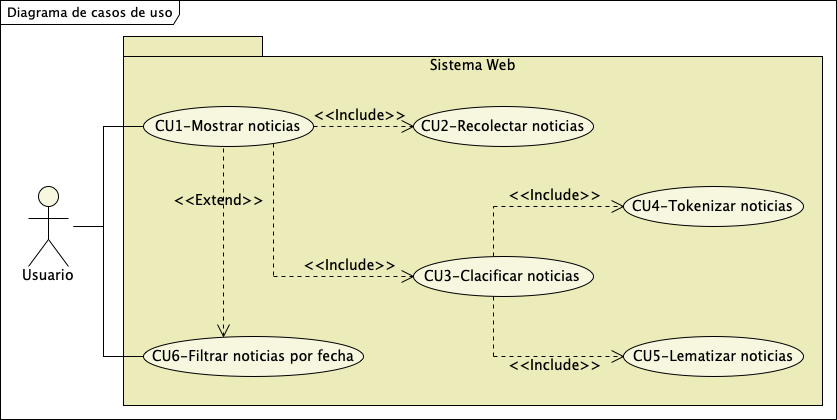
\includegraphics[scale=.4]{imagenes/Diagramas/CasosDeuso/CasosDeuso}
%  \caption{Diagrama de casos de uso}
%  \label{fig:DCU}
%\end{figure}


{\setlength{\parindent}{0pt}%Con este comando eliminos la indexación de cada párrafo%
  
  \newpage
  \Tlabel{CU1}\Tsubsection{CU1 Seleccionar sección}

%================================Intriodcucción==================================%
%----------------------Resumen-----------------------------------%
\begin{large}
	\textbf{Resumen}\\
\end{large}

Brinda al usuario un punto de acceso para elegir una sección; Las clasificaciones son, \textbf{Ciencia y técnología}, \textbf{Política}, \textbf{Deportes},  y \textbf{Economía} en cada una se podrá consultar noticias, artículos y publicaciones dentro de un intervalo de tiempo específico; La fuente de información será un diccionario de los sitios web mas consultados y confiables en México. Cabe mencionar que el intervalo de tiempo por defecto es la fecha actual que se ha ingresa al portal.\\

\begin{large}
	\textbf{Descripción}\\
\end{large}

%=====================================Tabla 1====================================%

\begin{tabular}{|l|l|}

%-----------------------Ecanbezado-----------------------------------%
	\hline
	\multicolumn{1}{| >{\columncolor{black}}l|}{ \textcolor{myWhite}{\textbf{Caso de uso: }} }&
	\multicolumn{1}{| >{\columncolor{black}}l|}{ \textcolor{myWhite}{CU1 Seleccionar sección} }\\
	\hline

%-----------------------Actor----------------------------------------%
	\textbf{Actor:} & 	Usuario	\\
	\hline

%-----------------------Propósito------------------------------------%
	\textbf{Propósito:} & Proporcionar una herramienta para acceder \\
	&a los diferentes tipos de clasificaciones disponibles.\\
	\hline

%----------------------Entradas--------------------------------%
	\textbf{Entradas:} & Ninguna. \\
	\hline

%-----------------------Salidas--------------------------------------%
	\textbf{Salidas:} &$\bullet$ \textit{Fecha inicio}\\
	&$\bullet$ \textit{Feha fin}\\
	&$\bullet$ \Tref{MSG1}{MSG1 Catálago vacio}\\
	\hline

%-----------------------Precondiciones-------------------------------%
	\textbf{Precondición:} & El catálogo \textbf{Direcciones web} debe estar poblado.\\
	\hline

%-----------------------Postcondiciones------------------------------%

%---------Post 1----------%
	\textbf{Postcondiciones:} &$\bullet$ El usario tendrá la facultad de buscar noticias\\
	&\ \ de la sección elegida\\
%---------Post 2----------%
	&$\bullet$ El usario tendrá la facultad de establecer un \\
	&\ \ intervalo de tiempo para buscar los artículos\\
	\hline

%-----------------------Reglas de negocio----------------------------%
	\textbf{Reglas de negocio:} &$\bullet$ \RNref{RN2}{Lenguaje de direcciones web} \\
	&$\bullet$ \RNref{RN7}{Perido preestablecido}\\
	\hline

%---------------------------Errores----------------------------------%

%------Error 1----------%
	\textbf{Errores:} & $\bullet$ \TError{CU1}{Uno} Cuando el  catálogo \textbf{Direcciones web}\\
	&\ \ no contiene información se muestra el mensaje\\
	&\ \  \Tref{MSG1}{MSG1 Catálago vacio}, fin del caso de uso\\
%------Error 2----------%
	&$\bullet$ \TError{CU1}{Dos} Cuando los sitios proporcionados no se\\
	&\ \ \ encuentran redactados en lenguaje  español se\\
	&\ \ muestra el mensaje \Tref{MSG2}{MSG2 Lenguaje de sitio}, fin\\
	&\ \ del caso de uso\\
	\hline

%-------------------------Autor--------------------------------------%
	\textbf{Autor:} & Carlos Andres Hernandez Gomez \\
	\hline
\end{tabular}\\\\

%============================Trayectorias========================================%

%-----------------------Trayectoria Principal-----------------------%


\begin{large}
	\textbf{Trayectoria principal}\\
\end{large}	

\begin{enumerate}[1.]
	
	\item \actor Selecciona una opción de la pantalla \Tref{UI1}{UI1 Inicio}; \textbf{Política}, \textbf{Economía}, \textbf{Deportes} o \textbf{Ciencia}. 
	
	\item \sistema Obtiene el catálogo \textbf{Direcciones web}.
	
	\item \sistema Verifica que el catálogo \textbf{Direcciones web} contenga información. \TEref{CU1}{Uno}
	
	\item \sistema Verifica que al menos un sitio cumpla con la regla de negocio \RNref{RN2}{Lenguaje de direcciones web}. \TEref{CU1}{Dos}

	\item \sistema Obtiene la fecha actual.

	\item \sistema \label{CU1:FechaI}Calcula el campo \textbf{Fecha incio} y \textbf{Fecha fin} deacuerdo a la regla de negocio \RNref{RN7}{Perido preestablecido}.

	\item \label{CU1:Pantalla}\sistema Muestra deshabilitado y con fechas los campos \textbf{Fecha inicio} y \textbf{Fecha fin} con lo antes calculado, como se visualiza en la pantalla \Tref{UI2}{UI2 Sección política}.
	
	\item \finCU	

\end{enumerate}


%================================Puntos de extención=============================%


%--------------------Puntos de extención 1------------------------%
\textbf{Causa de la extensión:} El actor desea consultar las noticias de una sección.\\
\textbf{Región de la trayectorioa:} Paso \ref{CU1:Pantalla} de la trayectoria principal.\\
\textbf{Extiende a :} \Tref{CU2}{CU2 Buscar noticia}.\\\\




  \newpage
  \Tlabel{CU2}\Tsubsection{CU2 Buscar noticias}

\begin{large}
	\textbf{Resumen}\\
\end{large}

Permite al actor realizar una busqueda de noticias correspondiente a cada tipo clasificación, ya sea \textbf{Política}, \textbf{Deportes}, \textbf{Ciencia} o \textbf{Economía}; El sitio muestra 15 noticias ordenadas de forma descendente deacuerdo a la fecha de difusión; Cada artículo contiene el \textbf{Título} , la \textbf{Fecha de publicación},un \textbf{Link} el cual direcciona a la página fuentey de contar con ello  un \textbf{Resumen de la información}.\\

\begin{large}
\textbf{Descripción}\\
\end{large}

\begin{tabular}{|l|l|}
\hline
\multicolumn{1}{| >{\columncolor{black}}l|}{ \textcolor{myWhite}{\textbf{Caso de uso: }} }&
\multicolumn{1}{| >{\columncolor{black}}l|}{ \textcolor{myWhite}{CU2 Buscar noticias} }\\
\hline
\textbf{Actor:} & 	Usuario	\\
\hline

\textbf{Propósito:} & Proporcionar una herramienta para  recolectar y clasificar\\
&noticias de una sección específica.\\
\hline

\textbf{Entradas:} &$\bullet$ \textit{Fecha inicio}\\
&$\bullet$ \textit{Feha fin}\\
\hline

\textbf{Salidas:}&Noticias clasificadas; De cada una se muestra:\\
&\ \ $\bullet$ \textbf{Título}\\
&\ \ $\bullet$ \textbf{Nombre de la página fuente}\\
&\ \ $\bullet$ \textbf{Link al artículo}\\
&\ \ $\bullet$ \textbf{Fecha de difusión}\\
&\ \ $\bullet$ \textbf{Resumen}\\
\hline

\textbf{Precondición:} & El campo \textbf{Fecha inicio} y \textbf{Fecha fin} deben contener\\
&información.\\
\hline

\textbf{Postcondiciones:} &$\bullet$ El usario tendrá la facultad de consultar las noticias\\
&$\bullet$ El usario tendrá la facultad de acceder a los sitios web\\
&\ \ de las noticias recolectadas\\
\hline

\textbf{Reglas de negocio:} &$\bullet$ \RNref{RN11}{Orden de publicación}\\
&$\bullet$ \RNref{RN8}{Campos obligatorios}\\
&$\bullet$ \RNref{RN12}{Formato de fecha}\\
&$\bullet$ \RNref{RN6}{Periodo válido}\\
&$\bullet$ \RNref{RN7}{Limite de periodo}\\

\hline

\textbf{Errores:} & Ninguno.\\
\hline

\textbf{Autor:} & Carlos Andres Hernandez Gomez \\
\hline
\end{tabular}\\\\

%%--------------------Trayectoria Principal-----------
\begin{large}
\textbf{Trayectoria principal}\\
\end{large}	

\begin{enumerate}[1.]

\item \actor Da click en el botón \textbf{Buscar} de la pantalla \Tref{UI2}{UI2 Sección política}. \TAref{A}

\item \sistema Verifica la regla de negocio \RNref{RN8}{Campos obligatorios}

\item \sistema 

\item \sistema Incluye el caso de uso \Tref{CU3}{CU3 Recolectar noticas}.

\item \sistema \label{CU2:ClasificarN}Incluye el caso de uso \Tref{CU4}{CU4 Calasificar noticias}.

\item \sistema \label{CU2:DatosN}Obtiene de cada noticia clasificada en el paso \ref{CU2:ClasificarN} de la trayectoria principal el \textbf{Título}, \textbf{Nombre de la página fuente}, \textbf{Link al artículo}, \textbf{Fecha de difusión} y de contar con ello el \textbf{Resumen}.

\item \sistema \label{CU2:OrdenaN}Ordena de forma descendente las noticias clasificadas del paso \ref{CU2:ClasificarN} de la trayectoria principal deacuerdo a su fecha de difusión.

\item \sistema Muestra 15 noticias de las ordenadas, deacuerdo a la regla de negocio \RNref{RN11}{Orden de publicación} con la información obtenida en el paso \ref{CU2:DatosN} de la trayectoria principal, como se visualiza en la pantalla \Tref{UI3}{UI3 Resultados de búsqueda} 

\item \actor \label{CU2:Consulta}Consulta la información.

\item \finCU	
\end{enumerate}


%%--------------------trayectoria Alternativa A----------
\begin{large}
\Talterna{A}\\
\end{large}	
\textbf{Condición:} \textit{El actor ha presionado el botón \textbf{Cambiar periodo}}

\begin{enumerate}[{A-}1.]

\item \sistema 
\item \finCU	

\end{enumerate}




  \newpage
  \Tlabel{CU3}\Tsubsection{CU3 Calasificar noticias}

\begin{large}
	\textbf{Resumen}\\
\end{large}

Texto.\\

\begin{large}
	\textbf{Descripción}\\
\end{large}

\begin{tabular}{|l|l|}
	\hline
	\multicolumn{1}{| >{\columncolor{black}}l|}{ \textcolor{myWhite}{\textbf{Caso de uso: }} }&
	\multicolumn{1}{| >{\columncolor{black}}l|}{ \textcolor{myWhite}{CU-1 Recolectar noticias} }\\
	\hline
	\textbf{Actor:} & 	Lorem Ipsum	\\
	\hline
	\textbf{Propósito:} & Lorem Ipsum \\
	\hline
	\textbf{Entradas:} & Lorem Ipsum \\
	\hline
	\textbf{Salidas:} & Lorem Ipsum\\
	\hline
	\textbf{Precondición:} & Lorem Ipsum \\
	\hline
	\textbf{Postcondiciones:} & Lorem Ipsum \\
	\hline
	\textbf{Reglas de negocio:} & Lorem Ipsum \\
	\hline
	\textbf{Errores:} & Lorem Ipsum \\
	\hline
	\textbf{Autor:} & Lorem Ipsum \\
	\hline
\end{tabular}\\\\

%--------------------Trayectoria Principal-----------%


\begin{large}
	\textbf{Trayectoria principal}\\
\end{large}	

\begin{enumerate}[1.]
	\item \actor lorem ipsum
	\item \sistema lorem ipsum
	\item \sistema lorem ipsum
	\item \sistema lorem ipsum
	\item \finCU	
\end{enumerate}


%--------------------trayectoria Alternatia A---------%

\begin{large}
	\textbf{Trayectoria alternativa A:}\\
\end{large}	
\textbf{Condición:} \textit{Se escribe la condición}
\begin{enumerate}[{A-}1.]

	\item \actor lorem ipsum
	\item \sistema lorem ipsum
	\item \finTA	

\end{enumerate}


%--------------------trayectoria Alternatia b---------%
\begin{large}
	\textbf{Trayectoria alternativa B:}\\
\end{large}	
\textbf{Condición:} \textit{Se escribe la condición}

\begin{enumerate}[{B-}1.]

	\item \actor lorem ipsum
	\item \sistema lorem ipsum
	\item \finTA	

\end{enumerate}


%--------------------Puntos de extención--------------------%

\begin{large}
	\textbf{Puntos de extensión}\\
\end{large}	

\textbf{Causa de la extensión:} Lorem ipsum\\
\textbf{Región de la trayectorioa:} Lorem ipsum\\
\textbf{Extiende a :} Lorem ipsum\\\\

\textbf{Causa de la extensión:} Lorem ipsum\\
\textbf{Región de la trayectorioa:} Lorem ipsum\\
\textbf{Extiende a :} Lorem ipsum\\


  \newpage
  \Tsubsection{CU4 Cambio de periodo}

%================================Intriodcucción==================================%
%----------------------Resumen-----------------------------------%
\begin{large}
	\textbf{Resumen}\\
\end{large}

Texto.\\

\begin{large}
	\textbf{Descripción}\\
\end{large} 

%=====================================Tabla 1====================================%

\begin{tabular}{|l|l|}
%-----------------------Ecanbezado-----------------------------------%
	\hline
	\multicolumn{1}{| >{\columncolor{black}}l|}{ \textcolor{myWhite}{\textbf{Caso de uso: }} }&
	\multicolumn{1}{| >{\columncolor{black}}l|}{ \textcolor{myWhite}{CU-1 Recolectar noticias} }\\
	\hline
%-----------------------Actor----------------------------------------%
	\textbf{Actor:} & 	Lorem Ipsum	\\
	\hline

%-----------------------Propósito------------------------------------%

	\textbf{Propósito:} & Lorem Ipsum \\
	\hline

%----------------------Entradas--------------------------------------%

	\textbf{Entradas:} & Lorem Ipsum \\
	\hline

%-----------------------Salidas--------------------------------------%

	\textbf{Salidas:} & Lorem Ipsum\\
	\hline

%-----------------------Precondiciones-------------------------------%

	\textbf{Precondición:} & Lorem Ipsum \\
	\hline
%-----------------------Postcondiciones------------------------------%

	\textbf{Postcondiciones:} & Lorem Ipsum \\
	\hline
%-----------------------Reglas de negocio----------------------------%

	\textbf{Reglas de negocio:} & Lorem Ipsum \\
	\hline

%---------------------------Errores----------------------------------%
	\textbf{Errores:} & Lorem Ipsum \\
	\hline
%-------------------------Autor--------------------------------------%
	\textbf{Autor:} & Lorem Ipsum \\
	\hline
\end{tabular}\\\\



%============================Trayectorias========================================%

%-----------------------Trayectoria Principal-----------------------%


\begin{large}
	\textbf{Trayectoria principal}\\
\end{large}	

\begin{enumerate}[1.]
	\item \actor lorem ipsum
	\item \sistema lorem ipsum
	\item \sistema lorem ipsum
	\item \sistema lorem ipsum
	\item \finCU	
\end{enumerate}


%-------------------------trayectoria Alternativa A-----------------%

\begin{large}
	\textbf{Trayectoria alternativa A:}\\
\end{large}	
\textbf{Condición:} \textit{Se escribe la condición}
\begin{enumerate}[{A-}1.]

	\item \actor lorem ipsum
	\item \sistema lorem ipsum
	\item \finTA	

\end{enumerate}


%----------------------trayectoria Alternativa B-------------------%
\begin{large}
	\textbf{Trayectoria alternativa B:}\\
\end{large}	
\textbf{Condición:} \textit{Se escribe la condición}

\begin{enumerate}[{B-}1.]

	\item \actor lorem ipsum
	\item \sistema lorem ipsum
	\item \finTA	

\end{enumerate}


%================================Puntos de extención=============================%


\begin{large}
	\textbf{Puntos de extensión}\\
\end{large}	

%--------------------Puntos de extención 1------------------------%
\textbf{Causa de la extensión:} Lorem ipsum\\
\textbf{Región de la trayectorioa:} Lorem ipsum\\
\textbf{Extiende a :} Lorem ipsum\\\\

%--------------------Puntos de extención 2------------------------%
\textbf{Causa de la extensión:} Lorem ipsum\\
\textbf{Región de la trayectorioa:} Lorem ipsum\\
\textbf{Extiende a :} Lorem ipsum\\


  \newpage
  \Tlabel{CU5}\Tsubsection{CU5 Ingrear a sitio web}


%================================Intriodcucción==================================%
%----------------------Resumen-----------------------------------%
\begin{large}
	\textbf{Resumen}\\
\end{large}

Permite al usuario acceder al portal web de las noticias mostradas.\\

\begin{large}
	\textbf{Descripción}\\
\end{large} 

%=====================================Tabla 1====================================%

\begin{tabular}{|l|l|}
%-----------------------Ecanbezado-----------------------------------%
	\hline
	\multicolumn{1}{| >{\columncolor{black}}l|}{ \textcolor{myWhite}{\textbf{Caso de uso: }} }&
	\multicolumn{1}{| >{\columncolor{black}}l|}{ \textcolor{myWhite}{CU7 Ingresar a sitio web} }\\
	\hline
%-----------------------Actor----------------------------------------%
	\textbf{Actor:} & Usuario.\\
	\hline

%-----------------------Propósito------------------------------------%

	\textbf{Propósito:} & Brindar un punto de acceso a los sitios web\\
	&que han proporcionado la información.\\
	\hline

%----------------------Entradas--------------------------------------%

	\textbf{Entradas:} & URL:Es seleccionado con el mouse.\\
	\hline

%-----------------------Salidas--------------------------------------%

	\textbf{Salidas:} &$\bullet$ Sitio web de la URL seleccionada\\
	&$\bullet$ \Tref{MSG8}{MSG8 Fallo al ingresar a sitio web}\\
	\hline

%-----------------------Precondiciones-------------------------------%

	\textbf{Precondición:} & Debe existir almenos una noticia mostrada\\
	& en el portal.\\
	\hline
%-----------------------Postcondiciones------------------------------%

	\textbf{Postcondiciones:} & El usario tendra la facultad de visualizar la\\ 
	&noticia completa.\\
	\hline
%-----------------------Reglas de negocio----------------------------%

	\textbf{Reglas de negocio:} & Ninguna.\\
	\hline

%---------------------------Errores----------------------------------%
	\textbf{Errores:} &\TError{CU7}{Uno} Cuando no es posible ingresar al sitio\\
	&\ web seleccionado, se muestra el mensaje \Tref{MSG8}{MSG8}\\
	&\ \Tref{MSG8}{Fallo al ingresar a sitio web} en la pantalla\\
	&\ \Tref{UI3}{UI3 Resultados de búsqueda}, fin del caso de uso.\\
	\hline
%-------------------------Autor--------------------------------------%
	\textbf{Autor:} & Carlos Andres Hernandez Gomez\\
	\hline
\end{tabular}\\\\



%============================Trayectorias========================================%

%-----------------------Trayectoria Principal-----------------------%


\begin{large}
	\textbf{Trayectoria principal}\\
\end{large}	

\begin{enumerate}[1.]
	\item \actor Solicita ver la noticia completa dando click en la \textbf{URL} de la publicación deseada, en la pantalla \Tref{UI3}{UI3 Resultados de búsqueda}.
	\item \sistema Abre una ventana en el navegador y en ella se direcciona a la URL seleccionada. \TEref{CU7}{Uno}
	\item \sistema Muestra la pantalla \Tref{UI4}{UI4 Página de sitio web}
	\item \finCU	
\end{enumerate}




%================================Puntos de extención=============================%





}

%------------------------Mensajes----------------------------------%

\section{Mensajes}
  
  %------------------MSG1-----------------------%
     \Mline{MSG1}{Catálago vacio}
    \begin{itemize}
      \item \textbf{Tipo:} Error. 
      \item \textbf{Objetivo:}  Dar a conocer que no se tiene las lígas a los sitios web.
      \item \textbf{Redacción:} El catálogo \textbf{Direcciones web} se encuentra vacio.
      \item \textbf{Referenciado por:} \Tref{CU1}{CU1 Seleccionar sección}\\
    \end{itemize}

  %------------------MSG2-----------------------%
     \Mline{MSG2}{Lenguaje de sitio}
    \begin{itemize}
      \item \textbf{Tipo:} Error. 
      \item \textbf{Objetivo:}  Dar a conocer que los sitios a los cuales desea ingresar, no están redactados en lenguaje español.
      \item \textbf{Redacción:} Los sitios no se encuentran en lenguaje español, por lo cual no serán consultados.
      \item \textbf{Referenciado por:} \Tref{CU1}{CU1 Seleccionar sección}\\
    \end{itemize}

  %------------------MSG3-----------------------%
     \Mline{MSG3}{Faltan campos obligatorios}
    \begin{itemize}
      \item \textbf{Tipo:} Error. 
      \item \textbf{Objetivo:}  Dar a conocer que hay campos obligatorios vacios.
      \item \textbf{Redacción:} Los campos marcados con * no pueden omitirse.
      \item \textbf{Referenciado por:} \Tref{CU2}{CU2 Buscar noticias}\\
    \end{itemize}

  %------------------MSG4-----------------------%
   \Mline{MSG4}{Formato de feha inválido}
  \begin{itemize}
    \item \textbf{Tipo:} Error. 
    \item \textbf{Objetivo:}  Informar que se ha ingrsado una fecha no válida.
    \item \textbf{Redacción:} Se ha ingresado una fecha inválida; El formato correcto es DD/MM/AAAA.
    \item \textbf{Referenciado por:} \Tref{CU2}{CU2 Buscar noticias}\\
  \end{itemize}

    %------------------MSG5-----------------------%
   \Mline{MSG5}{Periodo no válido}
  \begin{itemize}
    \item \textbf{Tipo:} Error. 
    \item \textbf{Objetivo:}  Informar que se ha ingrsado una un perido incongruente.
    \item \textbf{Redacción:} El periodo ingresado es incorrecto.
    \item \textbf{Referenciado por:} \Tref{CU2}{CU2 Buscar noticias}\\
  \end{itemize}

    %------------------MSG6-----------------------%
   \Mline{MSG6}{Lítimes fuera de rango}
  \begin{itemize}
    \item \textbf{Tipo:} Error. 
    \item \textbf{Objetivo:}  Informar que el intervalo de tiempo está fuera de los límites del sistema.
    \item \textbf{Redacción:} El periodo ingresado está fuera de los límites permitidos, la fecha debe estar entr 01/01/1990 y el día en curso.
    \item \textbf{Referenciado por:} \Tref{CU2}{CU2 Buscar noticias}\\
  \end{itemize}

  %--------------------------Descripción de pantallas ------------------%
\section{Pantallas}

\Tsubsection{UI1 Sitio} 

\Large{\textbf{Objetivo}}\\\\
\normalsize{Texto}\\

	

\Large{\textbf{Descripción}}\\
\normalsize{Texto}\\

\Large{\textbf{Comandos}}\\
\normalsize{}

\begin{itemize}
	\item Lorem ipsum
	\item Lorem ipsum
	\item Lorem ipsum
\end{itemize}


\Large{\textbf{Referencia}}\\\\
\normalsize{\Tref{CU1}{CU1 Mostrar noticias},\Tref{CU7}{CU7 Ingresar a sitio web}}

\begin{figure}[H]\Tlabel{UI1}
  \centering
	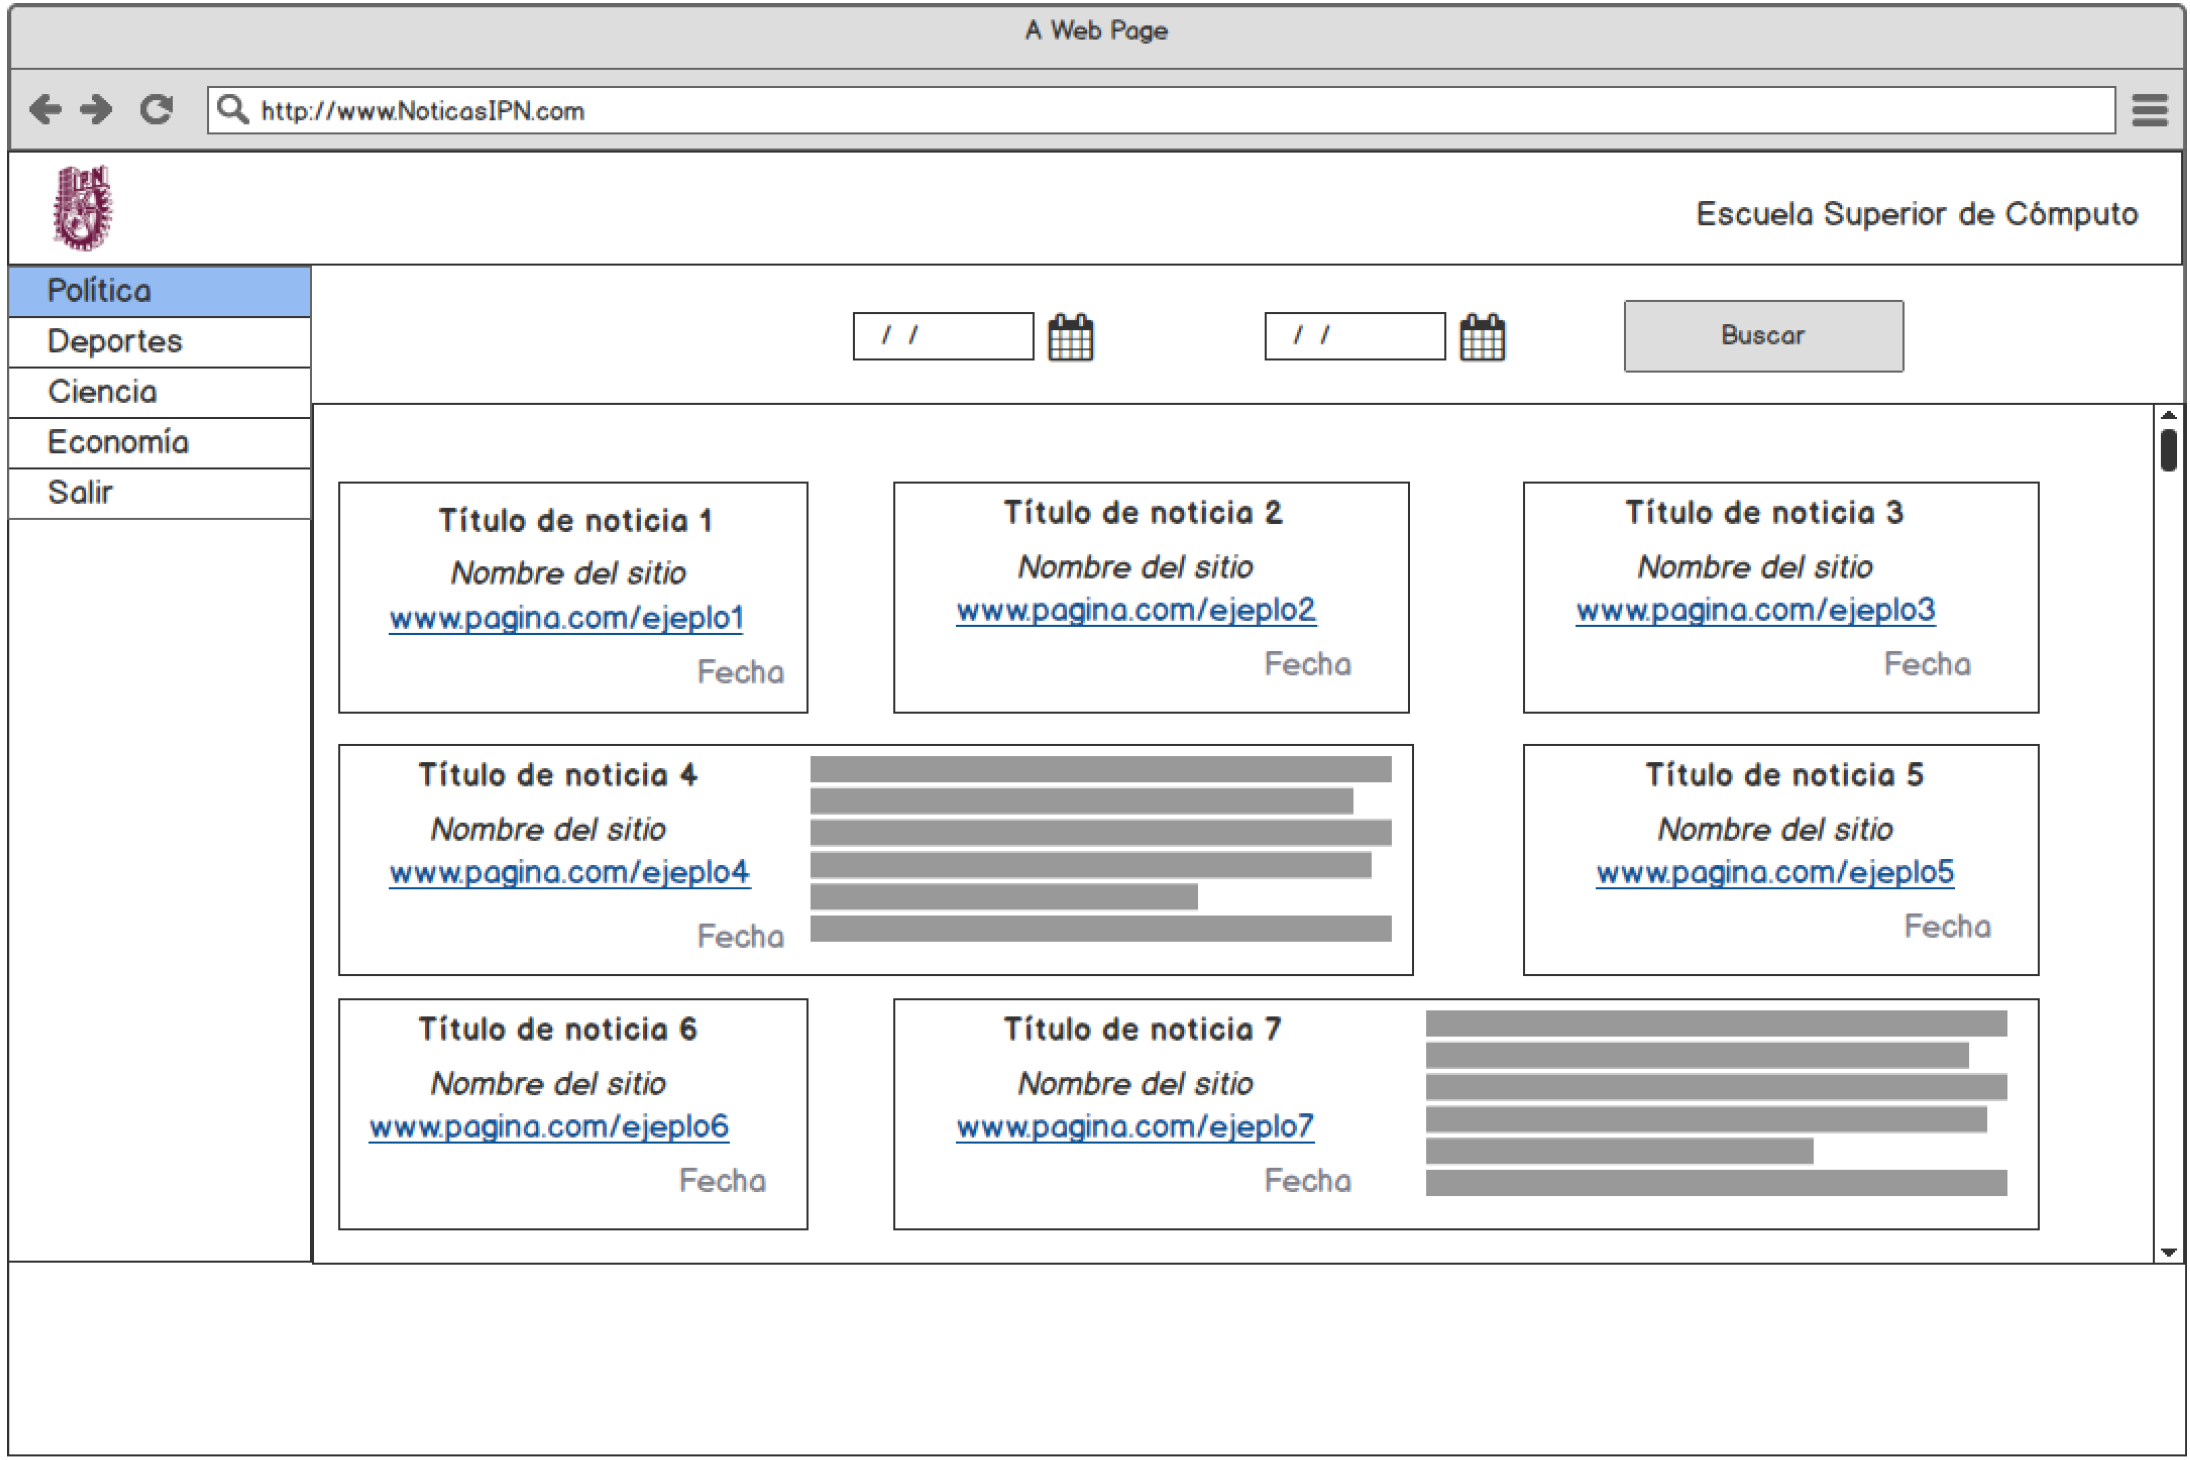
\includegraphics[scale=.35]{imagenes/Pantallas/UI1}
  \caption{Pantalla UI1 Inico}
  \label{fig:UI1}
\end{figure}



\begin{figure}[H]\Tlabel{UI2}
  \centering 
	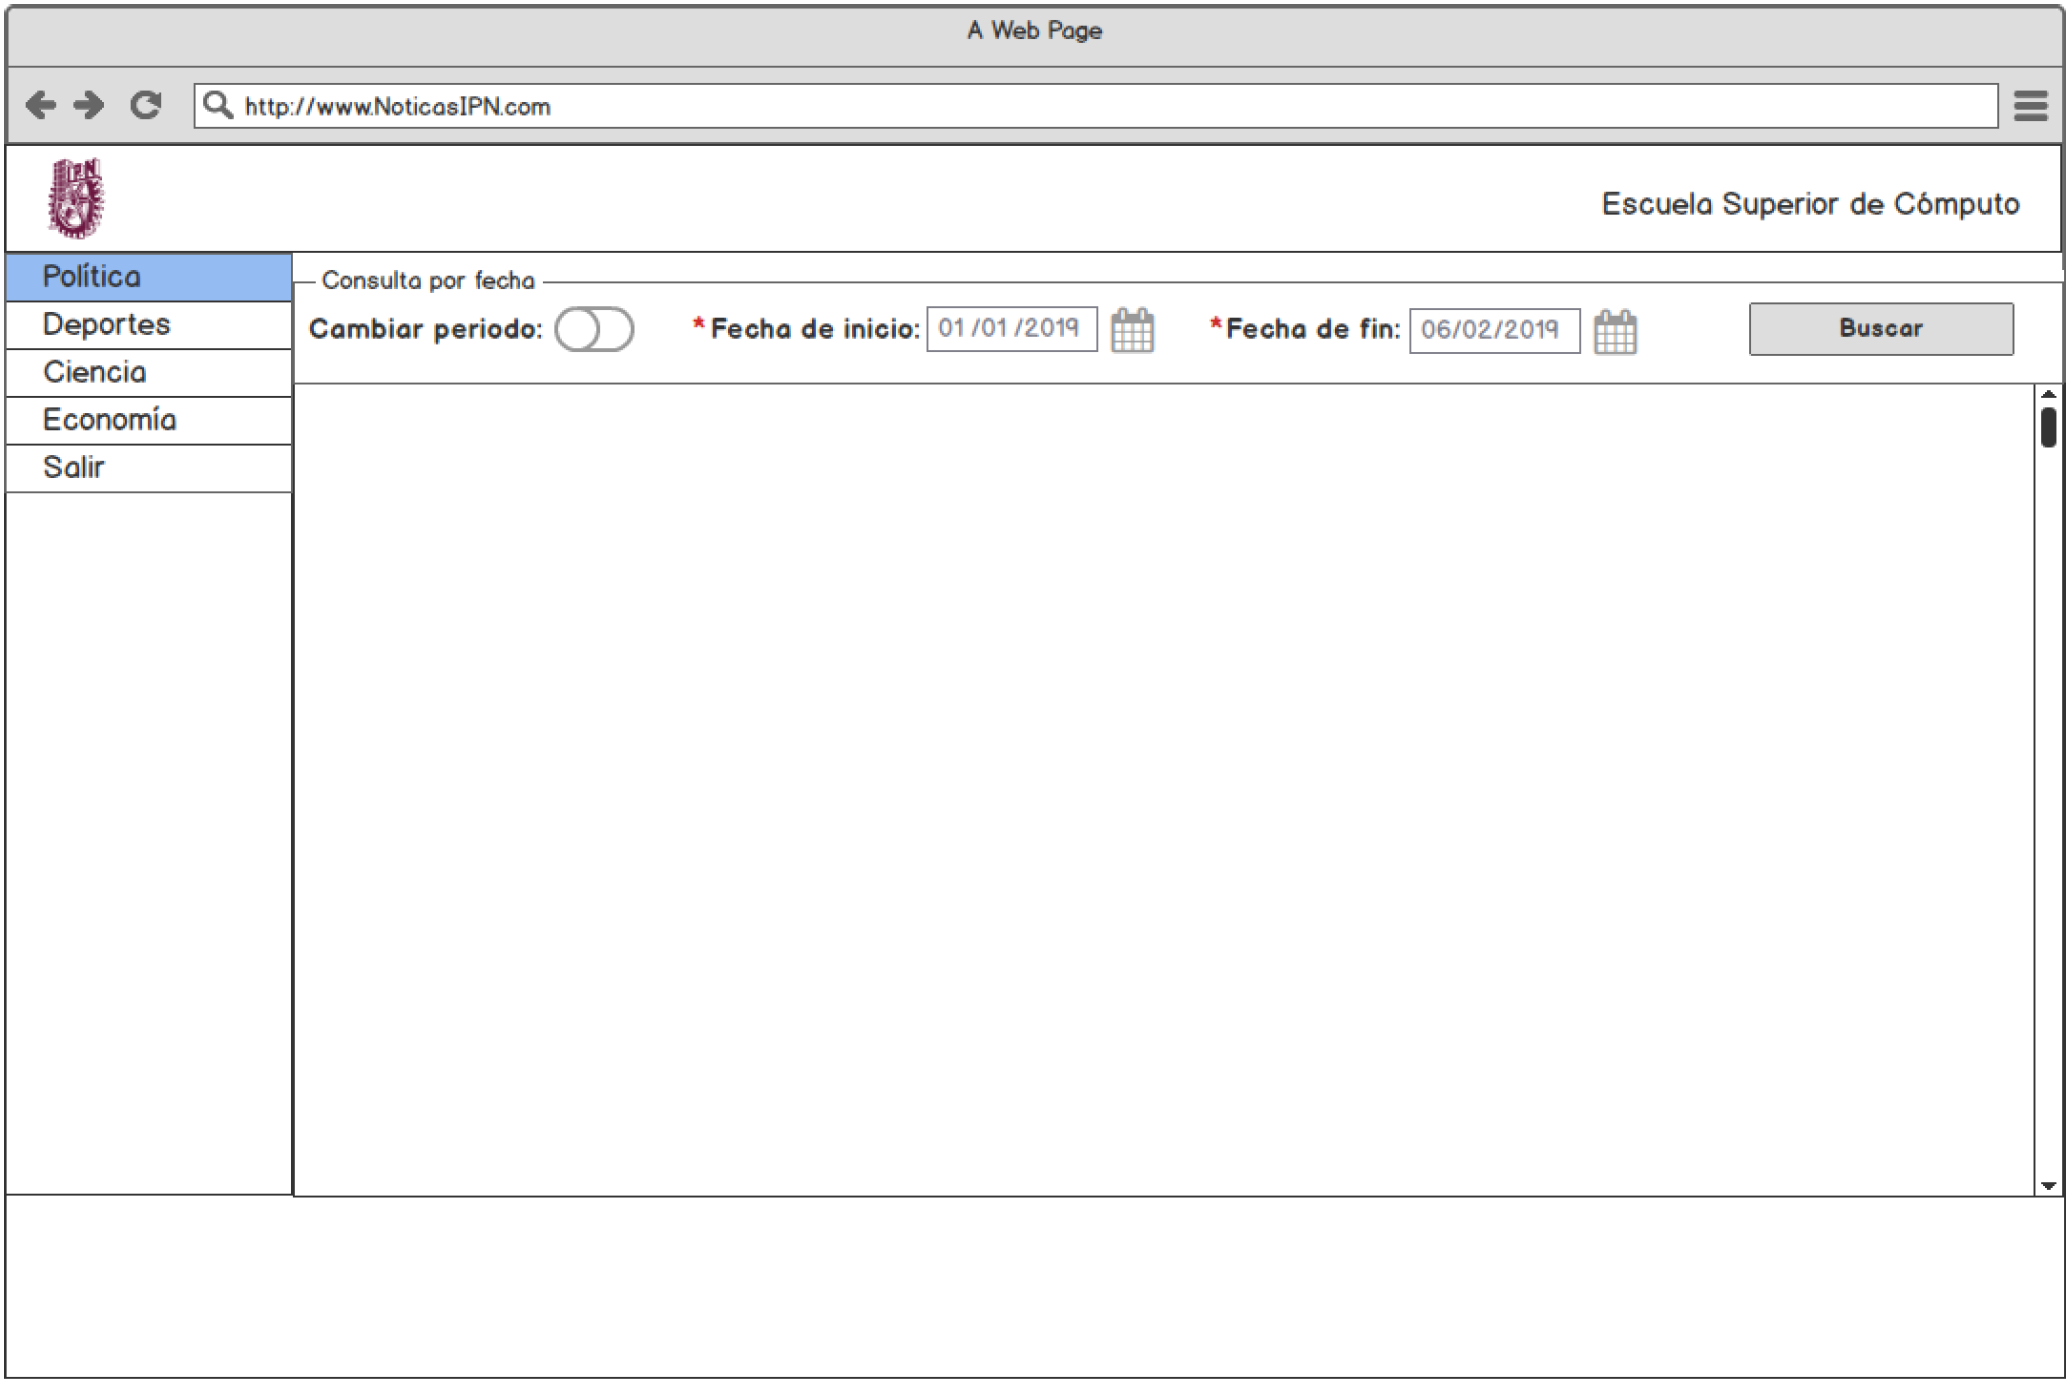
\includegraphics[scale=.35]{imagenes/Pantallas/UI2}
  \caption{Pantalla UI2 Sección política}
  \label{fig:UI2}
\end{figure}



\begin{figure}[H]\Tlabel{UI3}
  \centering
	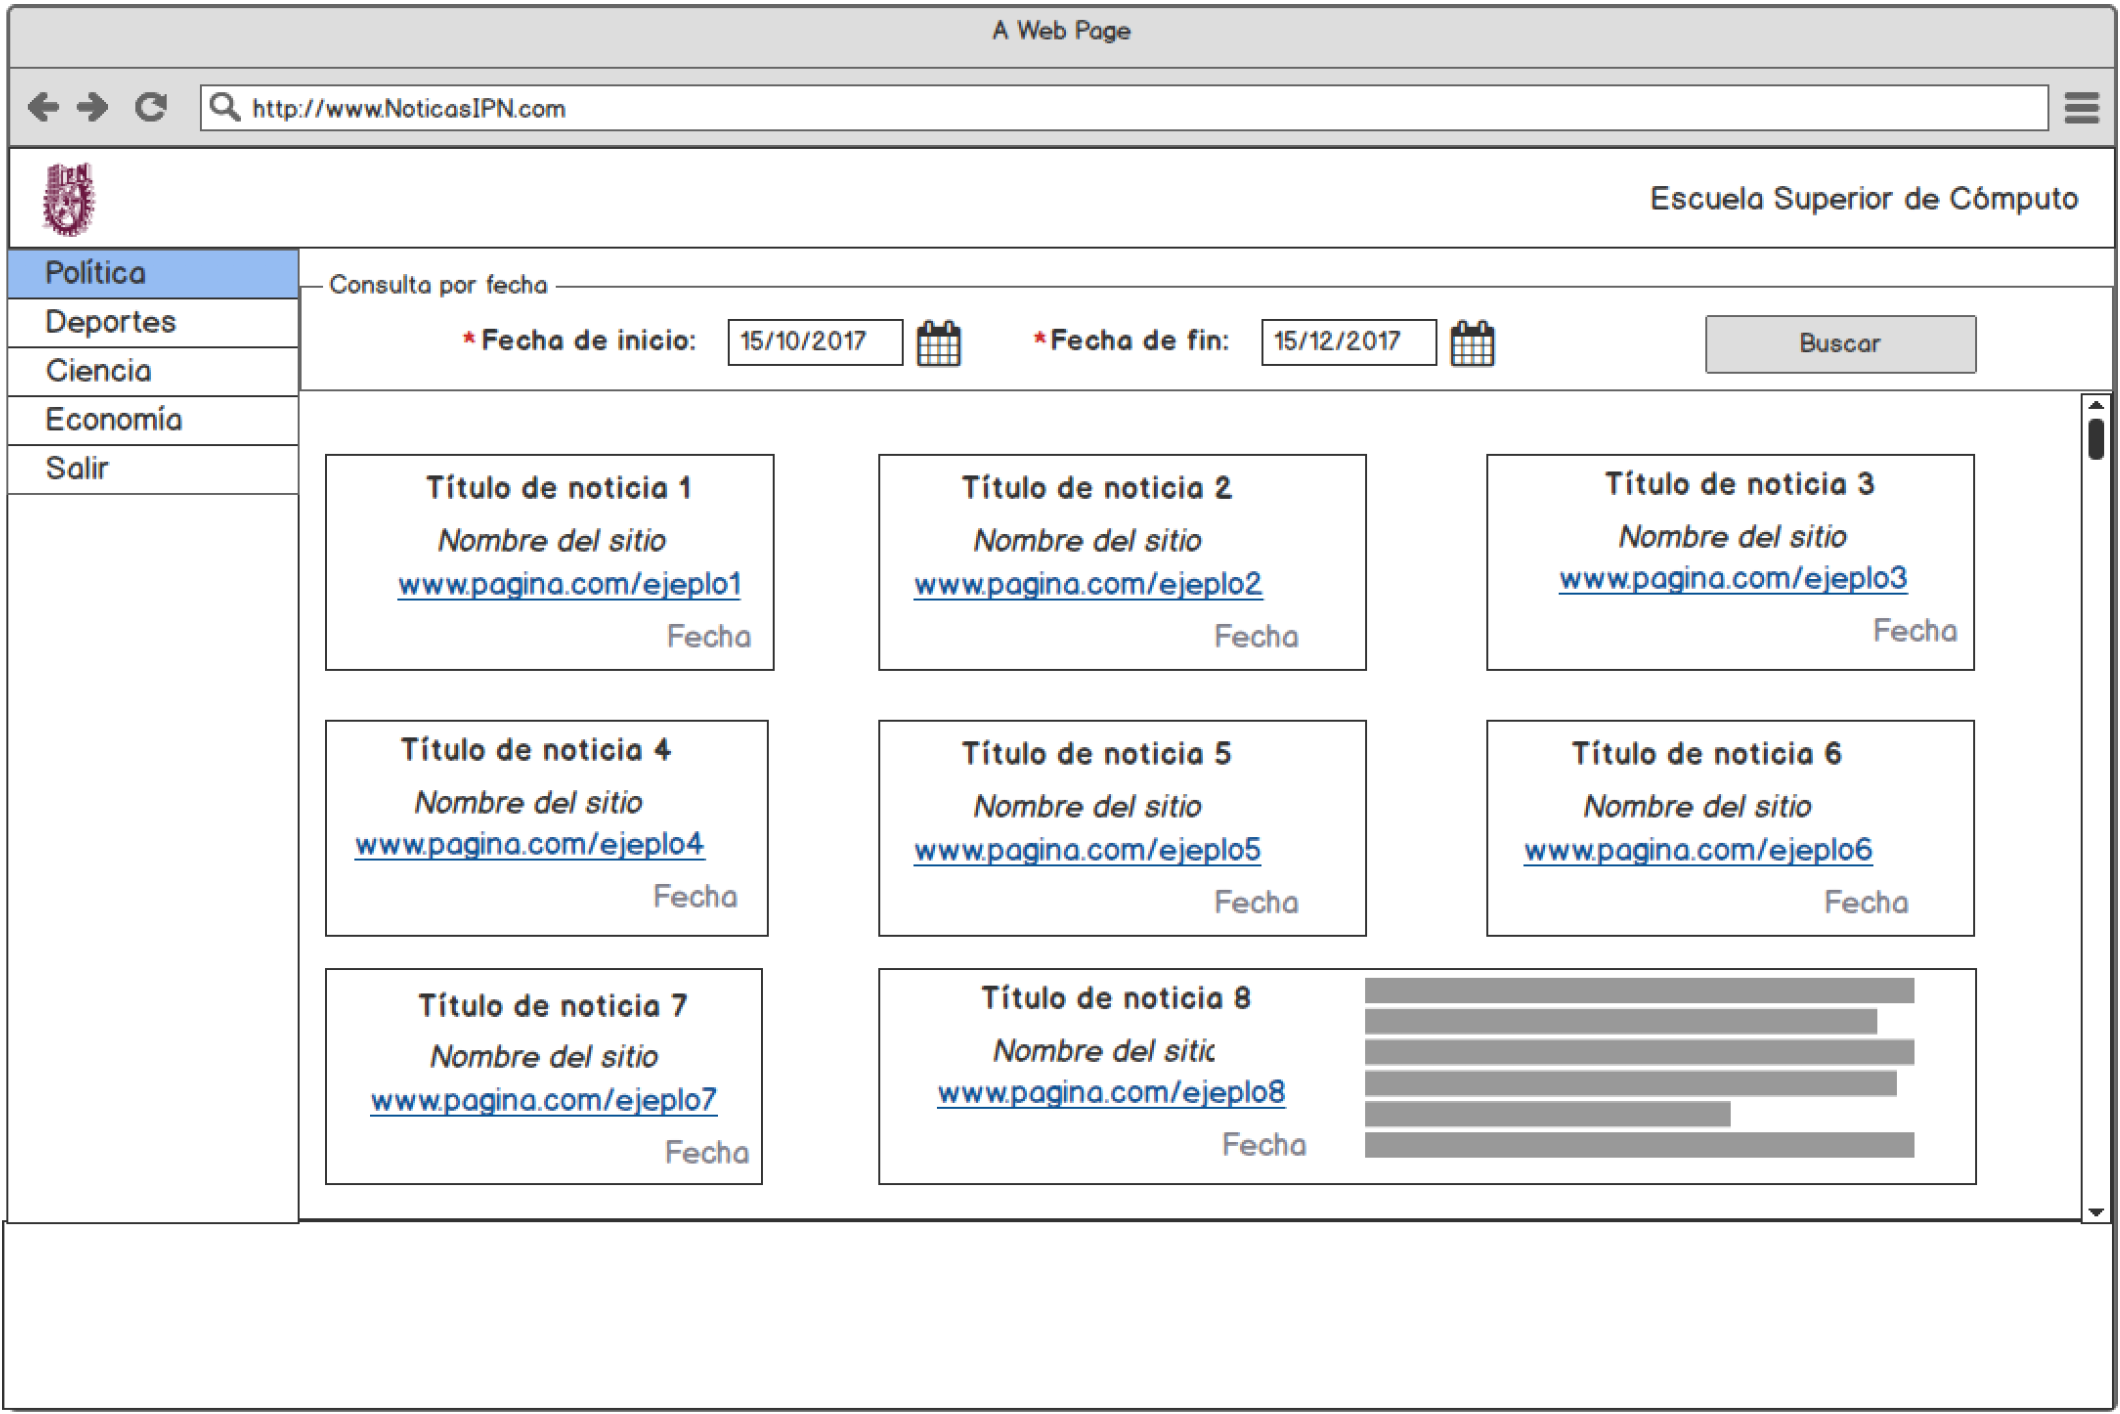
\includegraphics[scale=.35]{imagenes/Pantallas/UI3}
  \caption{Pantalla UI3 Cambio de periodo}
  \label{fig:UI3}
\end{figure}


\begin{figure}[H]\Tlabel{UI4}
  \centering
	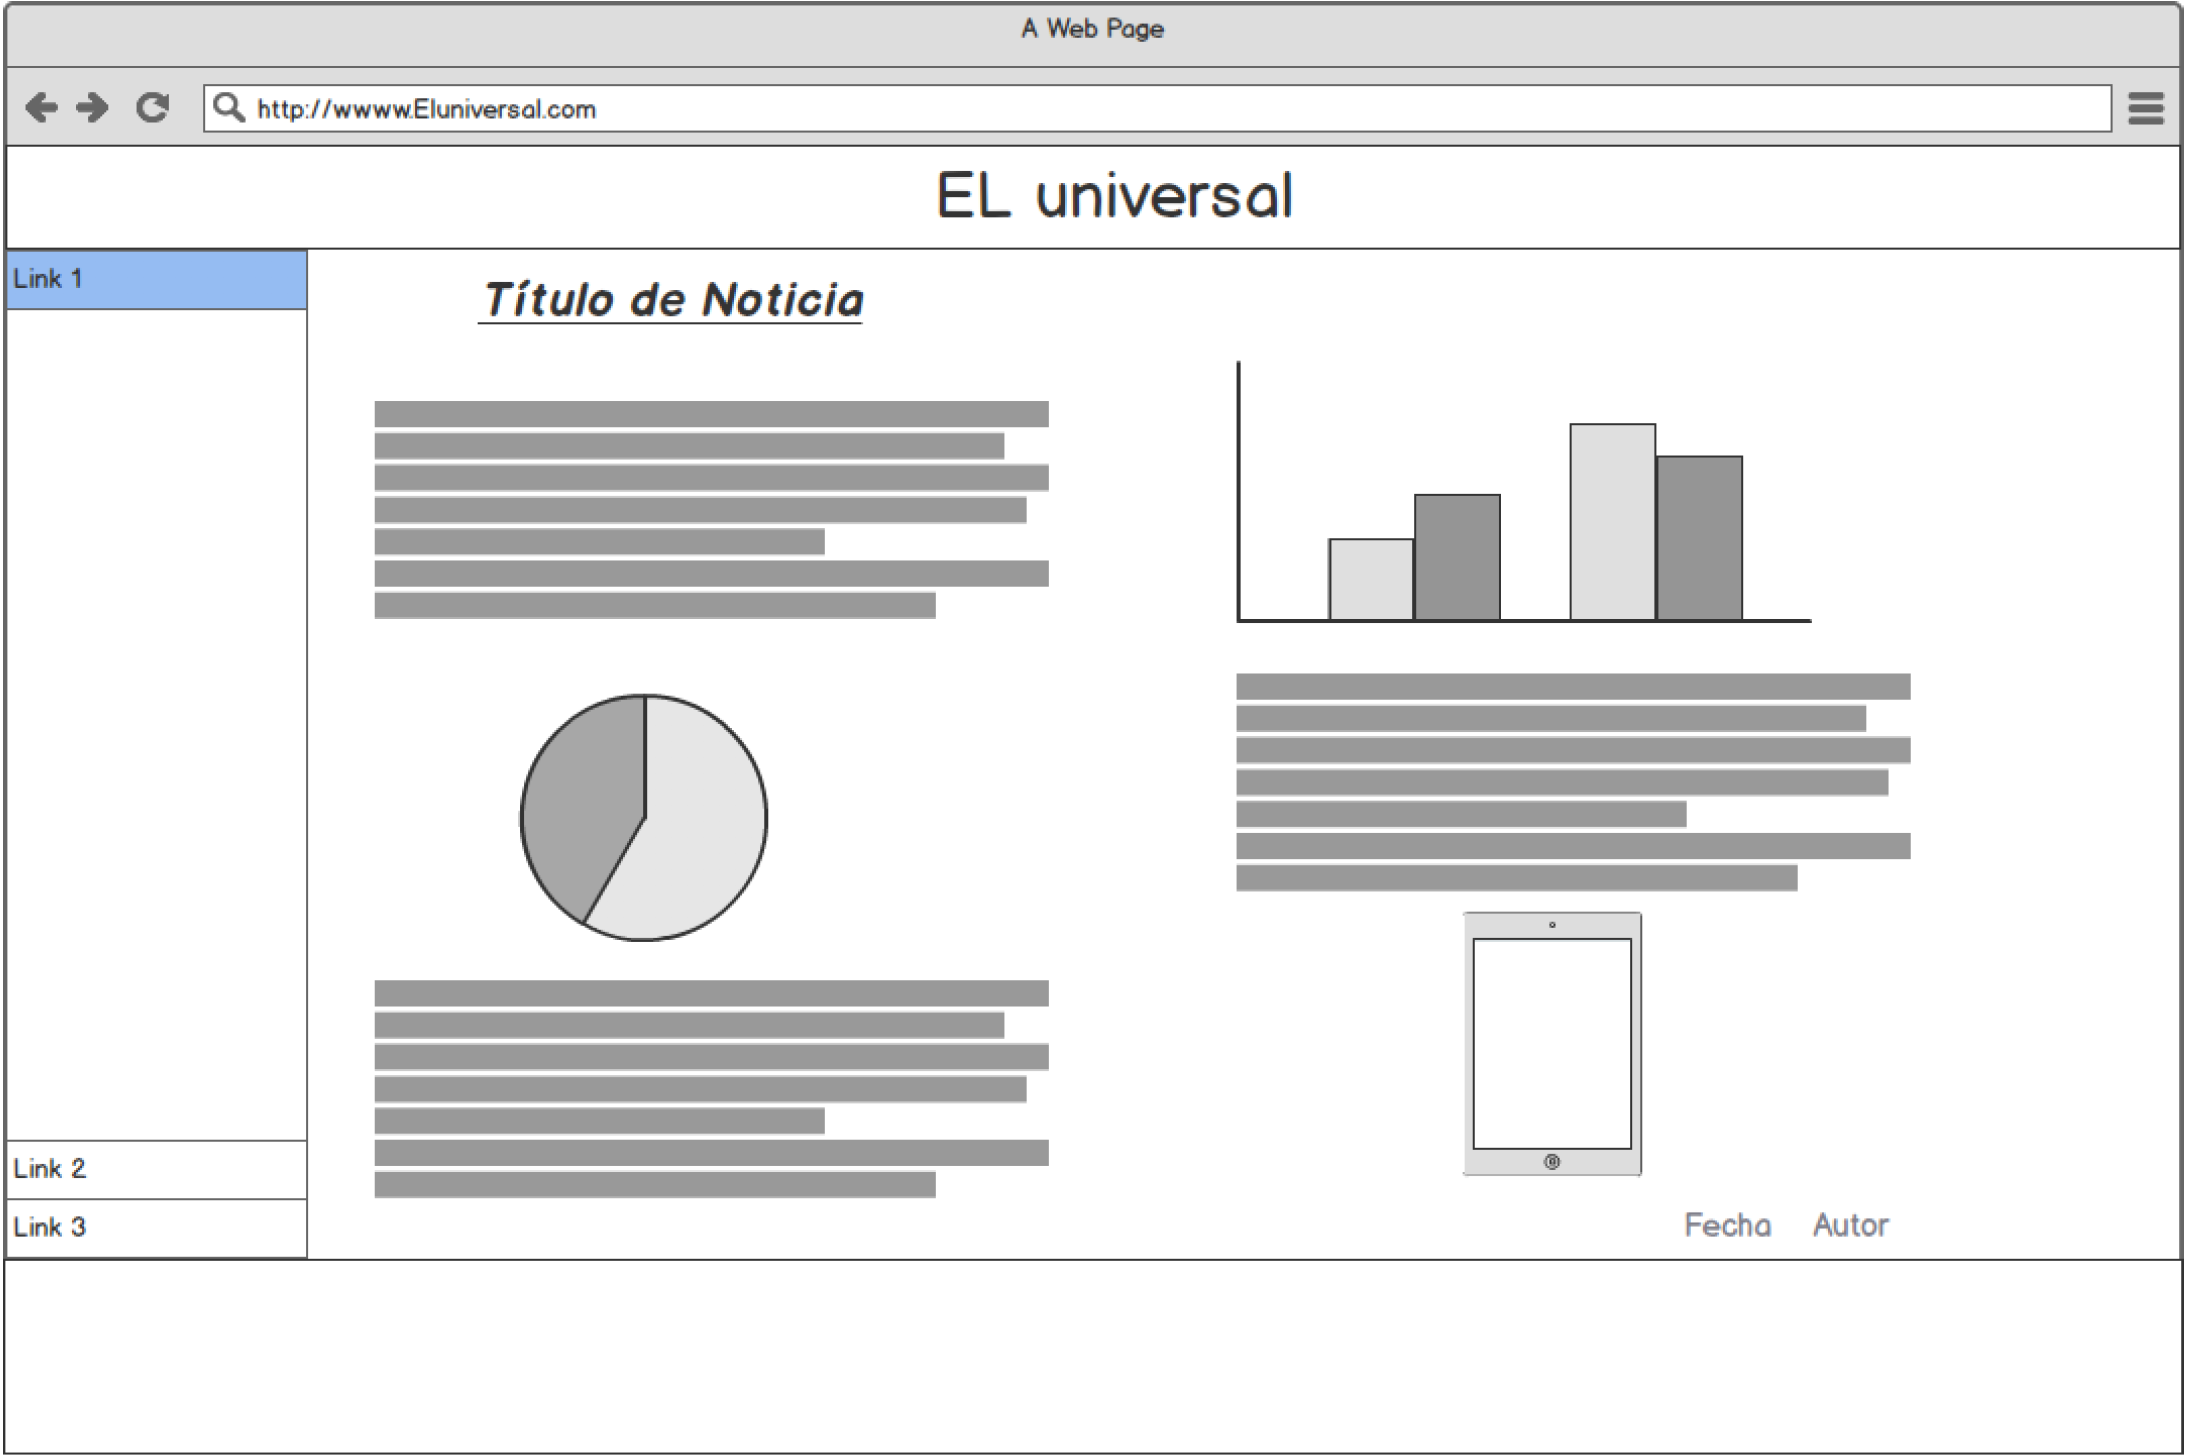
\includegraphics[scale=.35]{imagenes/Pantallas/UI4}
  \caption{Pantalla UI4 Página de sitio web}
  \label{fig:UI4}
\end{figure}
\newpage





